%==============================================================================
\chapter{Testes e resultados}\label{resultados}
%==============================================================================

Neste capítulo será mostrado qual foi o ambiente de teste, quais foram os experimentos e os seus respectivos resultados serão discutidos. No fim do capítulo os nossos resultados serão comparados com os resultados dos trabalhos relacionados. 


\section{Ambiente de teste}

\subsection{Bibliotecas}

A implementação do modelo neural foi realizada utilizando a linguagem Python com as seguintes bibliotecas:

\begin{itemize}
\item Theano (0.7.0 dev): Biblioteca que define, otimiza e avalia expressões matemáticas eficientemente. Executa em GPU caso desejado.
\item Keras (0.2.0): Biblioteca para aprendizagem profunda implementada sobre o Theano.
\item Numpy (1.10.1): Biblioteca usada para aplicações números. Possui implementações eficientes para operações com matrizes.
\item gensim (0.12.2): Biblioteca geralmente usada para aplicações de \ac{pln}. Possui um \textit{parser} dos \textit{dumps} da Wikipédia.
\end{itemize}


\subsection{Máquina}

Todos os experimentos foram executados na máquina com as configurações abaixo:

\begin{itemize}
\item Sistema operacional: Ubuntu 14.04 LTS
\item Processador: Intel Xeon X5690 CPU @ 3.47GHz $\times$ 24
\item Memória: 64GB 1333 MHz DDR3
\item Python 3.4.3
\end{itemize}


\section{Pré-processamento}

Nós transformamos palavras que têm uma ocorrência menor que a taxa de raridade em um símbolo especial chamado \texttt{<unknown>}. Também transformamos todos os dígitos em ``9'' para diminuir a esparsidade. Para ambos os modelos, nós utilizamos \textit{features} de capitalização, de prefixos e de sufixos.

Realizamos um treinamento não-supervisionado para gerar vetores distribuídos de palavras usando um \textit{dump} de artigos da Wikipédia disponível em: \url{https://dumps.wikimedia.org/ptwiki/latest/}. No total haviam cerca de 44 milhões de \textit{tokens} do \textit{dump} e após o treino haviam $618966$ vetores de palavras. Para o treino, consideramos a capitalização, acentuação e pontuação.

Com essas \textit{features}, espera-se que o número de erros para palavras fora do vocabulário seja menor, pois desse modo temos informações relevantes da palavra mesmo que ela não esteja no conjunto de treinamento. 

Para palavras que não estão no vocabulário do treinamento não-supervisionado, geramos um único vetor aleatório para elas (ou seja, as palavras compartilham o mesmo vetor).


\section{Hiperparâmetros}

Definimos como hiperparâmetros as variáveis que são mudadas em tempo de compilação pelo usuário e que influenciam na construção do modelo. Os hiperparâmetros escolhidos por nós se encontram na \autoref{tab:hiperparametrostab}.


\begin{table}[!htb]
\footnotesize
\centering
\caption{Hiperparâmetros para os modelos}
\label{tab:hiperparametrostab}
\begin{tabular}{m{6cm}P{4cm}P{4cm}}
  \toprule
  \textbf{Hiperparâmetro} & \textbf{Modelo recursivo} & \textbf{Modelo recorrente bidirecional}  \\
  \midrule
  Tamanho da janela de palavras  		& 5 & 11 \\
  Tamanho da janela de etiquetas     	& 5 & - \\
  Tamanho dos vetores de palavras  		& 50 & 50\\
  Tamanho dos vetores de capitalização 	& 7 & 7 \\
  Tamanho dos vetores de prefixos 		& 5 & 5 \\
  Tamanho dos vetores de sufixos 		& 5 & 5 \\
  Número de unidades ocultas 			& 250 & 250 \\
  Taxa de \textit{Dropout}			& 0.5 & 0.5 \\
  Taxa de aprendizagem 					& 1.0 & 1.0 \\
  Épocas de treinamento 				& 3 & 20 \\
  Tamanho do \textit{beam} 				& 3 & - \\
  Taxa de raridade						& 5 & 5 \\
  \bottomrule
\end{tabular}
\end{table}

O tamanho de janela e de etiquetas foi escolhido de modo empírico. Seguimos \cite{fonseca2015evaluating} e usamos $50$ para a dimensão dos vetores de palavras. O tamanho dos vetores de capitalização, de prefixos e de sufixos foram escolhidos de modo empírico. O número de unidades ocultas foi escolhido através de um \textit{trade-off} de tempo de execução e acurácia. A taxa de \textit{Dropout} foi escolhida de modo empírico. A taxa de aprendizagem foi deixada com o valor original do Keras. Definimos $3$ épocas de treinamento, porque o tempo de treinamento do modelo neural recursivo é alto, e além disso, não vimos diferença na diminuição do erro de validação após a terceira época. O tamanho do \textit{beam} utilizado foi o sugerido em \cite{shen2007guided}. 

O tamanho da janela de palavras no modelo recorrente bidirecional é maior pois queremos um maior contexto para ter informações à direita. O modelo recorrente bidirecional tem mais épocas porque seu treinamento é mais rápido e com mais épocas o erro de validação decresce. Os valores ``-'' para o recorrente bidirecional significa que os respectivos hiperparâmetros não existem para esse modelo.




\section{Resultados}

Utilizamos três \textit{córpus} para os experimentos: Mac-Morpho original \cite{aluisio2003account}; Mac-Morpho revisado \cite{fonseca2015evaluating} (conhecido também como Mac-Morpho versão 3); Tycho Brahe \cite{tychobrahe2010corpus}. Para todos esses \textit{córpus}, dividimos eles em dois conjuntos: Um conjunto de treino (80\%) e outro de validação (20\%). Fizemos o uso de vetores distribuídos de palavras aprendidos de forma não-supervisionada usando o Word2Vec, Wang2Vec e os vetores treinados por \citeonline{fonseca2015evaluating}. 

\subsection{Acurácia}

A acurácia mede a taxa de acertos e sua equação pode ser vista na \autoref{eq:acuraciaeq}, sendo $m$ o número de exemplos de treinamento, $\hat{y}$ a classe prevista pela rede neural, $y$ a classe correta e a função $equal(p, q)$ retorna $1$ se $p$ é igual a $q$, e $0$ caso contrário.

\begin{equation}\label{eq:acuraciaeq}
\frac{1}{m} \sum\limits_{i=1}^{m} equal(\hat{y}_i, y_i) 
\end{equation}

Foram obtidos resultados entre diferentes representações de palavras. Onde para cada representação de palavra foi calculada a acurácia entre palavras conhecidas, palavras desconhecidas (palavras que não estão no conjunto de treinamento e estão no conjunto de validação, considerando palavras raras como conhecidas), e também palavras ambíguas. Nós consideramos apenas a acurácia mais alta de uma determinada época sobre o conjunto de validação. 

Calculamos também a acurácia em relação a sentença inteira, onde consideramos uma sentença como correta se todas as palavras na sentença foram etiquetadas corretamente, e incorreta caso contrário. Essa métrica se encontra na coluna chamada ``Sentenças''.


Os resultados para o modelo neural recursivo podem ser vistos na \autoref{tab:acuraciam1_recur}, \autoref{tab:acuraciam3_recur} e \autoref{tab:acuraciatb_recur} para o Mac-Morpho original, Mac-Morpho revisado e para o Tycho Brahe, respectivamente.

\begin{table}[!htb]
\footnotesize
\centering
\caption{Modelo neural recursivo: Acurácia sobre o Mac-Morpho original}
\label{tab:acuraciam1_recur}
\begin{tabular}{m{2.5cm}P{2.2cm}P{2.2cm}P{2.2cm}P{2.2cm}P{2.2cm}}
  \toprule
  \textbf{Representação} & \textbf{Conhecidas (\%)}  & \textbf{Desconhecidas (\%)} & \textbf{Ambíguas (\%)} & \textbf{Total (\%)} & \textbf{Sentenças (\%)} \\
  \midrule
  Word2Vec  & 94.80 & 82.54 & 94.24 & 94.28 & 46.39  \\ % FEITO
  % GloVe     & 00.00 & 00.00 & 00.00 & 00.00 & 00.00  \\
  Wang2Vec  & 94.44 & 82.12 & 94.53 & 93.91 & 46.28  \\
  Fonseca 	& 95.92 & 86.77 & 95.26 & 95.53 & 47.39  \\
  \bottomrule
\end{tabular}
\end{table}


\begin{table}[!htb]
\footnotesize
\centering
\caption{Modelo neural recursivo: Acurácia sobre o Mac-Morpho revisado}
\label{tab:acuraciam3_recur}
\begin{tabular}{m{2.5cm}P{2.2cm}P{2.2cm}P{2.2cm}P{2.2cm}P{2.2cm}}
  \toprule
  \textbf{Representação} & \textbf{Conhecidas (\%)}  & \textbf{Desconhecidas (\%)} & \textbf{Ambíguas (\%)} & \textbf{Total (\%)} & \textbf{Sentenças (\%)} \\
  \midrule
  Word2Vec  & 94.13 & 80.99 & 93.02 & 93.78 & 42.14 \\ % FEITO (NO SERVIDOR)
  % GloVe     & 00.00 & 00.00 & 00.00 & 00.00 & 00.00 \\
  Wang2Vec  & 95.22 & 81.57 & 94.17 & 94.56 & 42.35 \\ % FEITO
  Fonseca 	& \textbf{96.12} & \textbf{88.32} & \textbf{96.44} & \textbf{95.79} & \textbf{47.28} \\ % FEITO
  \bottomrule
\end{tabular}
\end{table}



\begin{table}[!htb]
\footnotesize
\centering
\caption{Modelo neural recursivo: Acurácia sobre o Tycho Brahe}
\label{tab:acuraciatb_recur}
\begin{tabular}{m{2.5cm}P{2.2cm}P{2.2cm}P{2.2cm}P{2.2cm}P{2.2cm}}
  \toprule
  \textbf{Representação} & \textbf{Conhecidas (\%)}  & \textbf{Desconhecidas (\%)} & \textbf{Ambíguas (\%)} & \textbf{Total (\%)} & \textbf{Sentenças (\%)} \\
  \midrule
  Word2Vec  & 90.27 & 48.12 & 90.81 & 88.82 & 22.93  \\ % FEITO
  % GloVe     & 00.00 & 00.00 & 00.00 & 00.00 & 00.00  \\
  Wang2Vec  & 91.23 & 48.77 & 90.86 & 89.78 & 23.47  \\ % FEITO
  Fonseca 	& 89.74 & 47.75 & 89.24 & 88.31 & 19.54  \\ % FEITO
  \bottomrule
\end{tabular}
\end{table}


O modelo recursivo teve bastante dificuldade para classificar palavras desconhecidas, o que achávamos que não deveria ter acontecido, já que há o contexto de etiquetas que ajuda no momento da classificação. Acreditamos que isso aconteceu devido a ocorrência de \textit{underfitting}, uma vez que a acurácia de treinamento é baixa (para os padrões de \ac{pos} Tagging) e a de validação é mais baixa ainda. 


\begin{figure}[!htb]
  \caption{Acurácia de treinamento e validação para modelo recursivo usando o Wang2Vec}
  \label{fig:grafico_acc_epoca}
  \begin{center}
  \begin{tikzpicture}[scale=1]
    \begin{axis}[
      width=0.9\textwidth,
      height=0.42\textwidth,
      xmode=normal,
      ymode=normal,
      ymin=0.75,
      ymax=1.0,
      xmin=1,
      xmax=3,
      xtick=data,
      % ticks=both,
      xlabel=Época,
      ylabel=Acurácia (\%),
      legend pos=south east,
      legend cell align=left,
      % legend style={draw=none},
    ]
    \addplot+[green,mark=o] table [x=epoca,y=treino,header=true] {resultados/acuracia/recur_wang2vec_m1.txt};
    \addlegendentry{\tiny{Treinamento para Mac-Morpho original}}
    
    \addplot+[green,mark=square] table [x=epoca,y=val,header=true] {resultados/acuracia/recur_wang2vec_m1.txt};
    \addlegendentry{\tiny{Validação para Mac-Morpho original}}

    \addplot+[blue,mark=o] table [x=epoca,y=treino,header=true] {resultados/acuracia/recur_wang2vec_m3.txt};
    \addlegendentry{\tiny{Treinamento para Mac-Morpho revisado}}
    \addplot+[blue,mark=square] table [x=epoca,y=val,header=true] {resultados/acuracia/recur_wang2vec_m3.txt};
    \addlegendentry{\tiny{Validação para Mac-Morpho revisado}}

    \addplot+[red,mark=square] table [x=epoca,y=val,header=true] {resultados/acuracia/recur_wang2vec_tb.txt};
    \addlegendentry{\tiny{Validação para Tycho Brahe}}

    \addplot+[red,mark=o] table [x=epoca,y=treino,header=true] {resultados/acuracia/recur_wang2vec_tb.txt};
    \addlegendentry{\tiny{Treinamento para Tycho Brahe}}
    

  \end{axis}
  \end{tikzpicture}
\end{center}
\end{figure}


Através dos gráficos da acurácia de treinamento e validação pelo número de épocas para o modelo neural recursivo, mostrado na \autoref{fig:grafico_acc_epoca}, podemos ver que ele sofre de \textit{underfitting}, onde a acurácia de treinamento e validação são baixas. Apesar do número de épocas ser pequeno, é possível ver através da imagem que o modelo não aumenta significativamente a acurácia da segunda época para a terceira.

A acurácia obtida no Tycho Brahe foi baixa quando comparada aos trabalhos relacionados. Acreditamos que isso pode ser influenciado pelo fato do conjunto de etiquetas desse \textit{córpus} ser maior, e também pelo fato do Tycho Brahe ter mais sentenças compridas do que o Mac-Morpho. 


% \begin{figure}[!htb]
% 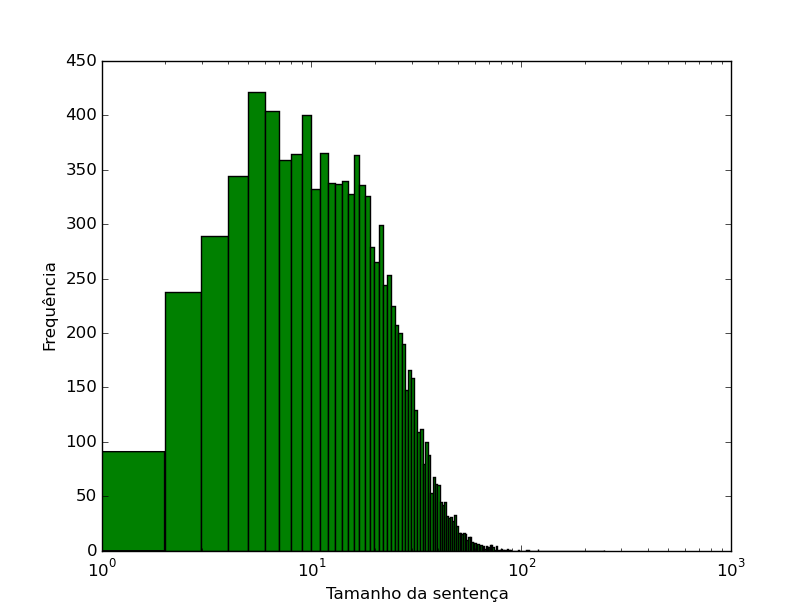
\includegraphics[width=1.0\textwidth]{img/distribuicao_macmorphov3_test.png} 
% \caption{}
% \end{figure}

% \begin{figure}[!htb]
% 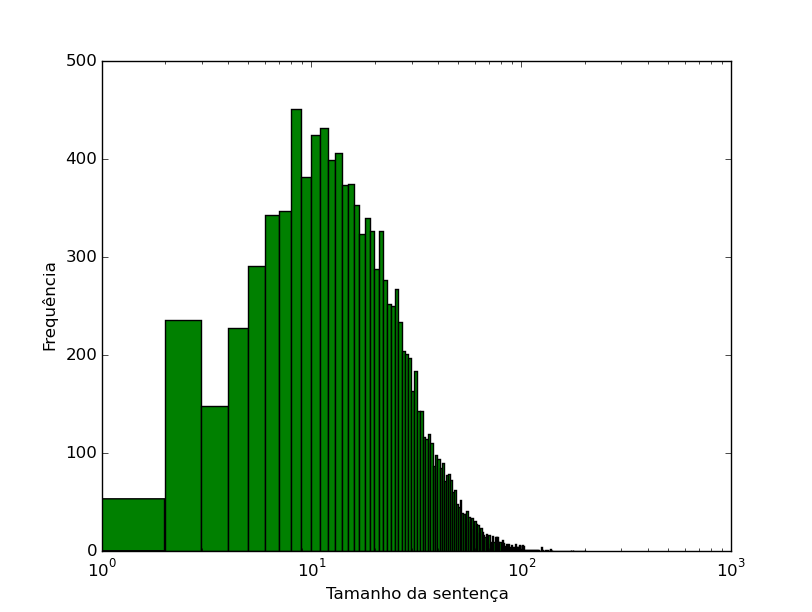
\includegraphics[width=1.0\textwidth]{img/distribuicao_tychobrahe_test.png} 
% \caption{Distribuição dos comprimentos das sentenças no conjunto de validação do Tycho Brahe} 
% \end{figure} 



A \autoref{fig:distribuicaocorpus1} e a \autoref{fig:distribuicaocorpus2} mostram, respectivamente, a distribuição dos comprimentos das sentenças no conjunto de validação do Mac-Morpho e do Tycho Brahe. Nela, é possível perceber que o Tycho Brahe tem mais sentenças com comprimento maior que $50$. Já o Mac-Morpho tem um maior número de sentenças com comprimento menor que $50$. Desse modo, um erro cometido na fase inicial do algoritmo de predição é levado adiante e afeta as outras classificações 

\begin{figure}[!htb]
  \caption{Distribuição dos comprimentos das sentenças}
  \begin{subfigure}[htb]{0.5\textwidth} 
     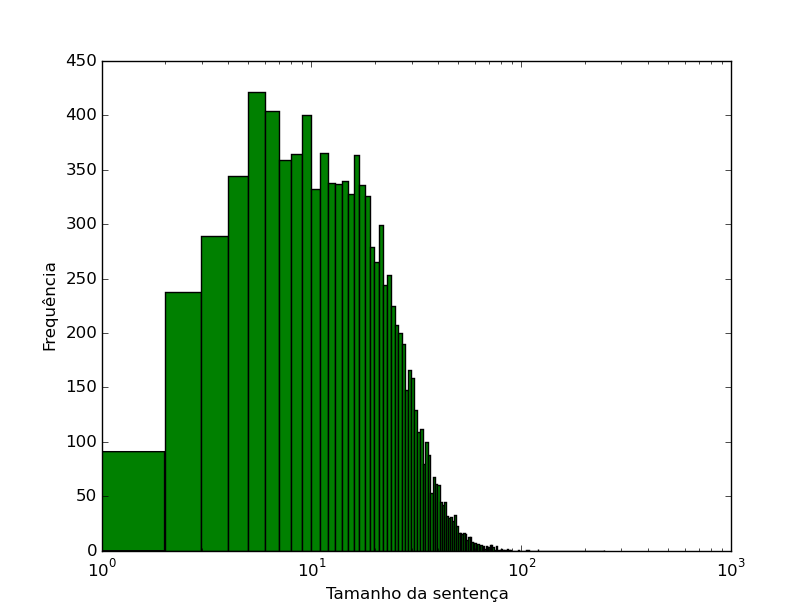
\includegraphics[width=\textwidth]{img/distribuicao_macmorphov3_test.png} 
    \caption{Mac-Morpho} \label{fig:distribuicaocorpus1}
  \end{subfigure} 
  %
  \begin{subfigure}[htb]{0.5\textwidth}
    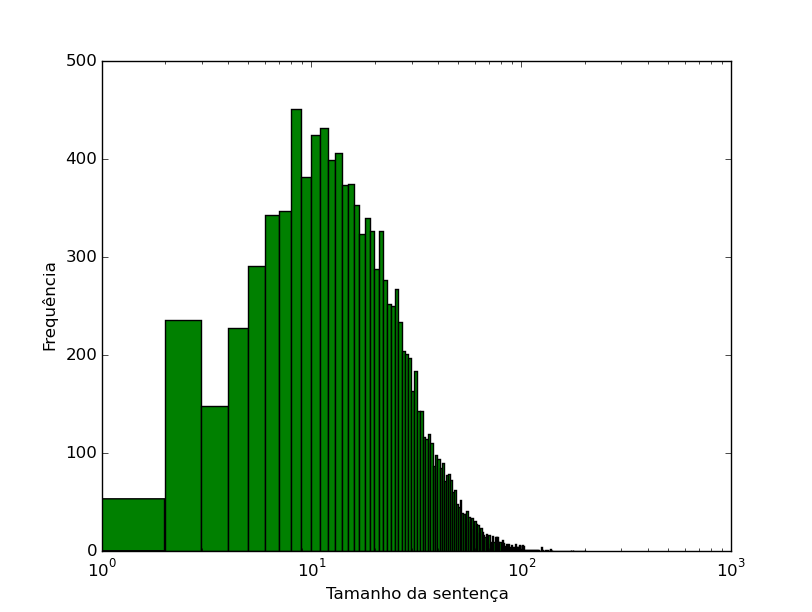
\includegraphics[width=\textwidth]{img/distribuicao_tychobrahe_test.png} 
    \caption{Tycho Brahe} \label{fig:distribuicaocorpus2}
  \end{subfigure} 
\end{figure}




Os resultados do modelo neural recorrente bidirecional podem ser encontrados na \autoref{tab:acuraciam1_bidir}, \autoref{tab:acuraciam3_bidir} e \autoref{tab:acuraciatb_bidir} para o Mac-Morpho original, Mac-Morpho revisado e para o Tycho Brahe, respectivamente.

\begin{table}[!htb]
\footnotesize
\centering
\caption{Modelo neural recorrente bidirecional: Acurácia sobre o Mac-Morpho original}
\label{tab:acuraciam1_bidir}
\begin{tabular}{m{2.5cm}P{2.2cm}P{2.2cm}P{2.2cm}P{2.2cm}P{2.2cm}}
  \toprule
  \textbf{Representação} & \textbf{Conhecidas (\%)}  & \textbf{Desconhecidas (\%)} & \textbf{Ambíguas (\%)} & \textbf{Total (\%)} & \textbf{Sentenças (\%)} \\
  \midrule
  Word2Vec  & 97.01 & 88.79 & 97.05 & 97.01 & 59.43  \\ % FEITO
  % GloVe     & 00.00 & 00.00 & 00.00 & 00.00 & 00.00  \\
  Wang2Vec  & 97.03 & 87.60 & 96.70 & 96.63 & 56.63  \\ % FEITO
  Fonseca 	& \textbf{97.60} & \textbf{92.63} & \textbf{97.25} & \textbf{97.37} & \textbf{66.38}	 \\ % FEITO
  \bottomrule
\end{tabular}
\end{table}


\begin{table}[!htb]
\footnotesize
\centering
\caption{Modelo neural recorrente bidirecional: Acurácia sobre o Mac-Morpho revisado}
\label{tab:acuraciam3_bidir}
\begin{tabular}{m{2.5cm}P{2.2cm}P{2.2cm}P{2.2cm}P{2.2cm}P{2.2cm}}
  \toprule
  \textbf{Representação} & \textbf{Conhecidas (\%)}  & \textbf{Desconhecidas (\%)} & \textbf{Ambíguas (\%)} & \textbf{Total (\%)} & \textbf{Sentenças (\%)} \\
  \midrule
  Word2Vec  & 96.92 & 87.28 & 96.30 & 96.45 & \textbf{57.03} \\ % FEITO
  % GloVe     & 00.00 & 00.00 & 00.00 & 00.00 & 00.00 \\
  Wang2Vec  & 97.33 & 90.03 & 96.50 & 96.99 & 56.04 \\ % FEITO
  Fonseca  	& \textbf{97.33} & \textbf{92.18} & \textbf{96.50} & \textbf{97.08} & 56.77 \\ % FEITO
  \bottomrule
\end{tabular}
\end{table}



\begin{table}[!htb]
\footnotesize
\centering
\caption{Modelo neural recorrente bidirecional: Acurácia sobre o Tycho Brahe}
\label{tab:acuraciatb_bidir}
\begin{tabular}{m{2.5cm}P{2.2cm}P{2.2cm}P{2.2cm}P{2.2cm}P{2.2cm}}
  \toprule
  \textbf{Representação} & \textbf{Conhecidas (\%)}  & \textbf{Desconhecidas (\%)} & \textbf{Ambíguas (\%)} & \textbf{Total (\%)} & \textbf{Sentenças (\%)} \\
  \midrule
  Word2Vec  & 96.42 & 65.45 & 95.85 & 95.53 & 57.54  \\ % FEITO
  % GloVe     & 00.00 & 00.00 & 00.00 & 00.00 & 00.00  \\
  Wang2Vec  & 96.33 & 68.07 & 95.37 & 95.36 & 58.91  \\ % FEITO
  Fonseca 	& \textbf{96.80} & \textbf{73.39} & \textbf{96.09} & \textbf{96.00} & \textbf{64.80}  \\ % FEITO
  \bottomrule
\end{tabular}
\end{table}



O modelo recorrente bidirecional funciona muito bem para a tarefa de \ac{pos} Tagging. Os resultados no Mac-Morpho original e no revisado mostram que nossas hipóteses (de longa dependência e contexto da direita) estavam corretas. Os resultados desses \textit{córpus} ficaram muito próximos dos estados-da-arte sem requerer muito esforço para criação de \textit{features} manualmente. 

A acurácia para palavras fora do vocabulário no Tycho Brahe continuou deixando a desejar nesse modelo. Temos duas hipóteses do porquê disso ter ocorrido: A primeira é a questão do tamanho da sentença; A segunda é a questão dos vetores de palavras utilizados. 


\begin{figure}[!htb]
  \caption{Taxa de erros por tamanho da sentença no Tycho Brahe}
  \label{fig:erroporsentenca}
  \begin{center}
  \begin{tikzpicture}[scale=1]
    \begin{axis}[
      width=0.9\textwidth,
      height=0.3\textwidth,
      xmode=normal, %log
      ymode=normal, %log
      ymin=0,
      ymax=1.05,
      xmin=1,
      xmax=144,
      % xtick=data,
      % ticks=both,
      xlabel=Tamanho da sentença,
      ylabel=Taxa de erros (\%),
      legend pos=south east,
      legend cell align=left,
      %legend style={draw=none},
    ]
    \addplot+[blue,thick,mark=none] table [x=tamanho,y=erro,header=true] {resultados/tamanho_sentencas/recur_wang2vec_tb.txt};
    \addlegendentry{\scriptsize{Recursivo/Wang2Vec}}
    \addplot+[red,thick,mark=none] table [x=tamanho,y=erro,header=true] {resultados/tamanho_sentencas/bidir_wang2vec_tb.txt};
    \addlegendentry{\scriptsize{Recorrente/Wang2Vec}}
  \end{axis}
  \end{tikzpicture}
\end{center}
\end{figure}


Para a primeira hipótese, a \autoref{fig:erroporsentenca} mostra que, para ambos os modelos, a taxa de erros do Tycho Brahe tem um crescimento significativo conforme o tamanho da sentença aumenta, sendo que o recursivo comete mais erros que o bidirecional. Entretanto, a gente não vê uma causa do porquê disso ocorrer. A verdade é que vários fatores podem influenciar esse comportamento, como por exemplo os hiperparâmetros, a precisão de ponto flutuante utilizada, e até a próprio modo de treinamento/predição. A \autoref{tab:tammediasentencas} mostra o tamanho média das sentenças em cada \textit{córpus}.



\begin{table}[!htb]
\footnotesize
\centering
\caption{Tamanho médio das sentenças}
\label{tab:tammediasentencas}
\begin{tabular}{lccc}
  \toprule
  \textbf{Conjunto} & \textbf{Mac-Morpho original (\%)}  & \textbf{Mac-Morpho revisado (\%)} & \textbf{Tycho Brahe (\%)} \\
  \midrule
  Treino & 19 & 19 & 22 \\ 
  Teste  & 17 & 17 & 22 \\ 
  \bottomrule
\end{tabular}
\end{table}


Com os dados da \autoref{tab:tammediasentencas} e usando as equações da análise de complexidade vistas no \autoref{modeloneuralrecursivo}, é possível ver que o tempo de treinamento e de predição para o Tycho Brahe foi maior que para o Mac-Morpho. Na prática, o tempo de treinamento e predição do modelo recursivo foi cerca de oito vezes maior do que o do modelo bidirecional.


\begin{equation} \label{eq:taxadevetoresnaoencontradoseq}
\frac{\mbox{\texttt{número de vetores não encontrados}}}{\mbox{\texttt{número de palavras no vocabulário}}}
\end{equation}

\begin{table}[!htb]
\footnotesize
\centering
\caption{Taxa de vetores não encontrados}
\label{tab:vetoresnaoencontrados}
\begin{tabular}{lP{3cm}P{3cm}P{3cm}}
  \toprule
  \textbf{Representação} & \textbf{Mac-Morpho original (\%)}  & \textbf{Mac-Morpho revisado (\%)} & \textbf{Tycho Brahe (\%)} \\
  \midrule
  Word2Vec  & 33.92 & 27.74 & 78.52 \\ 
  Wang2Vec  & 33.92 & 27.74 & 78.52 \\
  Fonseca 	& 39.33 & 32.12 & 93.98 \\
  \bottomrule
\end{tabular}
\end{table}


Para a segunda hipótese, podemos levar em consideração a taxa de vetores não encontrados, descrita na \autoref{eq:taxadevetoresnaoencontradoseq}, para cada \textit{córpus} e representação de palavras utilizada, isso pode ser visto na \autoref{tab:vetoresnaoencontrados}. 




Perceba que a taxa de vetores não encontrados para o Tycho Brahe é muito maior que para os outros \textit{córpus}. Além disso, é possível analisar que os vetores disponibilizados por \citeonline{fonseca2015evaluating} obtiveram a melhor acurácia na maioria dos casos. Isso foi porque eles foram treinados num \textit{córpus} com cerca de 240 milhões de \textit{tokens} numa junção de artigos da Wikipédia e publicações do portal G1 (\url{http://www.g1.com.br)}). Isso fez com que seus vetores ficassem mais precisos no contexto do Mac-Morpho (uma vez que o Mac-Morpho é uma compilação de textos jornalísticos publicados na Folha de São Paulo em 1994).

Podemos também analisar a taxa de ocorrência de vetores não encontrados através da \autoref{eq:taxadeocorrenciavets}. A \autoref{tab:vetoresnaoencontradosocorrencia} mostra os valores dessa taxa para os três \textit{córpus} utilizados para cada representação de palavras.

\begin{equation} \label{eq:taxadeocorrenciavets}
\frac{\mbox{\texttt{ocorrência de vetores não encontrados}}}{\mbox{\texttt{número de palavras no conjunto de (treinamento $\cup$ validação)}}}
\end{equation}


% MAC-MORPHO REVISADO + WANG2VEC:
% NUMBER OF OOV VECTORS: 7126 / 25688
% TOTAL OOV: 155247 / (728497 + 178373)

% MAC-MORPHO REVISADO + FONSECA:
% NUMBER OF OOV VECTORS: 8252  / 25688
% TOTAL OOV: 15684 / (728497 + 178373)

% MAC-MORPHO REVISADO + WORD2VEC:
% NUMBER OF OOV VECTORS: 7126 / 25688
% TOTAL OOV: 155247 / (728497 + 178373)


% TYCHO-BRAHE + WANG2VEC:
% NUMBER OF OOV VECTORS: 21606 / 27515
% TOTAL OOV: 190831 / (775602 + 259991)

% TYCHO-BRAHE + FONSECA:
% NUMBER OF OOV VECTORS: 25859 / 27515
% TOTAL OOV: 64471 / (775602 + 259991)

% TYCHO-BRAHE + WORD2VEC:
% NUMBER OF OOV VECTORS: 21606 / 27515
% TOTAL OOV: 190831 / (775602 + 259991)


% MAC-MORPHO ORIGINAL + WANG2VEC:
% NUMBER OF OOV VECTORS: 8715 / 25688
% TOTAL OOV: 190536 / (728497 + 178373)

% MAC-MORPHO ORIGINAL + FONSECA:
% NUMBER OF OOV VECTORS: 10104  / 25688
% TOTAL OOV: 19489 / (728497 + 178373)

% MAC-MORPHO ORIGINAL + WORD2VEC:
% NUMBER OF OOV VECTORS: 8715 / 25688
% TOTAL OOV: 190536 / (728497 + 178373)



\begin{table}[!htb]
\footnotesize
\centering
\caption{Taxa de ocorrência de vetores não encontrados}
\label{tab:vetoresnaoencontradosocorrencia}
\begin{tabular}{lP{3cm}P{3cm}P{3cm}}
  \toprule
  \textbf{Representação} & \textbf{Mac-Morpho original (\%)}  & \textbf{Mac-Morpho revisado (\%)} & \textbf{Tycho Brahe (\%)} \\
  \midrule
  Word2Vec  & 21.01 & 17.11 & 18.42 \\
  Wang2Vec  & 21.01 & 17.11 & 18.42 \\
  Fonseca 	& 2.14  & 1.72  & 6.22 \\ 
  \bottomrule
\end{tabular}
\end{table}

Através desses dados, é possível perceber que, por mais que o número de vetores fora do vocabulário seja maior para a representação dos vetores disponibilizados por \citeonline{fonseca2015evaluating}, essa representação ainda tem uma taxa muito menor de ocorrência de vetores não encontrados. Isso significa que nosso \textit{dump} da Wikipédia era bem distrbuído, porém não continha palavras que ocorrem frequentemente nos \textit{córpus} analisados. Essas tabelas fazem têm uma correlação direta com os resultados obtidos. Desse modo, acreditamos que isso foi o que mais influenciou os resultados.

Vale a pena comentar que as linhas dos Word2Vec e do Wang2Vec são iguais pois eles foram treinados sobre o mesmo \textit{dump} da Wikipédia.





% Em \cite{kepler2010variable} é mostrado que as palavras ``que'' e ``a'' são geralmente classificadas errado devido ao fato delas serem muito ambíguas. Por isso, para ter uma boa ideia dos erros do modelo, é bom analisar a matriz de confusão dessas palavras. A matriz de confusão da palavra ``que'' para o Mac-Morpho e pro Tycho Brahe usando o modelo recorrente bidirecional pode ser vistas na  \autoref{tab:confusaoquemm} e na \autoref{tab:confusaoquetb} (A linha é a referência e a coluna é a previsão).




% \begin{table}[!htb] 
% \caption{Matriz de confusão para ``que'' para o Mac-Morpho original usando os vetores disponibilizados por \citeonline{fonseca2015evaluating}} \label{tab:confusaoquemm}
% \scriptsize 
% \centering 
% \begin{BVerbatim}
%            |    P                             A                     |
%            |    R                             D                     |
%            |    O                             V                     |
%            |    -                             -                     |
%            |    K         P    P              K    P         A      |
%            |    S         R    R         N    S    R         D      |
%            |    -         O    O    P    P    -    O         V    P |
%            |    R         -    S    D    R    R    A    A    -    R |
%            |    E    K    K    U    E    O    E    D    D    K    E |
%            |    L    S    S    B    N    P    L    J    V    S    P |
% -----------+--------------------------------------------------------+
% PRO-KS-REL |<1685>  89   14    2    .    .    .    .    .    .    . |
%         KS |  101<1433>   1    2    .    .    .    .    1    .    . |
%     PRO-KS |   43   16  <92>   6    .    .    .    .    1    .    . |
%     PROSUB |    1    4    7  <12>   .    .    .    .    4    .    . |
%       PDEN |    2    9    .    .   <.>   .    .    .    .    .    . |
%      NPROP |    .    2    .    6    .   <.>   .    .    .    .    . |
% ADV-KS-REL |    6    .    .    .    .    .   <.>   .    .    .    . |
%     PROADJ |    2    1    .    1    .    .    .   <.>   .    .    . |
%        ADV |    .    3    .    .    .    .    .    .   <.>   .    . |
%     ADV-KS |    .    1    1    .    .    .    .    .    .   <.>   . |
%       PREP |    .    1    .    .    .    .    .    .    .    .   <.>|
% -----------+--------------------------------------------------------+
% \end{BVerbatim}
% \end{table}


% \begin{table}[!htb] 
% \caption{Matriz de confusão para ``que'' para o Tycho Brahe usando os vetores disponibilizados por \citeonline{fonseca2015evaluating}} \label{tab:confusaoquetb}
% \scriptsize 
% \centering 
% \begin{BVerbatim}
%      |    W         C                   W |
%      |    P         O                   D |
%      |    R         N    W    F         - |
%      |    O    C    J    D    W    D    P |
% -----+------------------------------------+
% WPRO |<5793> 329    8   22    .    .    . |
%    C |  861<3697>  11   25    .    .    . |
% CONJ |   89   80  <28>   1    .    .    . |
%   WD |   12   16    .  <77>   .    .    . |
%   FW |    .    1    .    .   <3>   .    . |
%    D |    .    2    .    .    .   <.>   . |
% WD-P |    .    .    .    1    .    .   <.>|
% -----+------------------------------------+
% \end{BVerbatim}
% \end{table}





\section{Comparação com trabalhos relacionados}

Juntamos os melhores resultados de cada trabalho relacionado e comparamos com os nossos melhores resultados para cada \textit{córpus}, isso pode ser visto na \autoref{tab:comparacaoresultados}. O melhor resultado para cada \textit{córpus} está destacado em negrito. 


\bgroup
\renewcommand{\arraystretch}{1.5}
\begin{table}[!htb]
\footnotesize
\centering
\caption{Comparação da acurácia dos resultados com trabalhos relacionados} \label{tab:comparacaoresultados}
\begin{tabular}{m{2.2cm}cclcclcc}
\toprule
\multicolumn{1}{c}{\textbf{\textit{Córpus}}} & \multicolumn{2}{c}{\textbf{Mac-Morpho original}} &  & \multicolumn{2}{c}{\textbf{Mac-Morpho revisado}} &  & \multicolumn{2}{c}{\textbf{Tycho Brahe}} \\ \cline{2-3} \cline{5-6} \cline{8-9} 
\multicolumn{1}{c}{}               & \textbf{Todas(\%)} & \textbf{FDV(\%)} &  & \textbf{Todas(\%)} & \textbf{FDV(\%)} &  & \textbf{Todas(\%)} &  \textbf{FDV(\%)} \\
\midrule
\citeonline{kepler2010variable}    &      -           &    -           &  &  -               &   -             &  &   96,29     &      71,60     \\
\citeonline{dos2014training}       &     97.47        &   92.49        &  &  -               &   -             &  &   \textbf{97.17}     &      \textbf{86.58}     \\
\citeonline{fonseca2015evaluating} & \textbf{97.57}   & \textbf{93.38} &  & \textbf{97.33}   &  \textbf{93.66} &  &   96.93     &      84.14     \\
Este trabalho                      &     97.37        &   92.63        &  &      97.08       &  92.18          &  &   96.00     &      73.39     \\
\bottomrule
\end{tabular}
\end{table}
\egroup


Conforme discutido na seção anterior, um dos motivos que levaram \citeonline{fonseca2015evaluating} conseguir bons resultados foi o tamanho do \textit{dump} que utilizaram para treinar os vetores distribuídos, assim como o fato de terem treinados sobre textos jornalísticos beneficiou o resultado para o Mac-Morpho. 

\citeonline{dos2014training} não utilizaram vetores distribuídos de palavras pré-treinados, mas criaram um modelo de palavras e de caracteres que ajudou para palavras fora do vocabulário. 

Nossos melhores resultados foram atingidos usando o modelo neural recorrente bidirecional. Eles estão bem próximos dos melhores resultados para cada \textit{córpus}, e levando em consideração que nosso \textit{dump} da Wikipédia era pequeno e não continha algumas palavras que ocorrem com frequência, o modelo bidirecional conseguiu ótimos resultados. Acreditamos que empregando um modelo de caracteres como feito por \citeonline{dos2014training} e aumentando o tamanho do \textit{dump} nos ajude a levantar a acurácia. 